\documentclass[../sherrill-Mix_thesis.tex]{subfiles}
\begin{document}
\chapter{Conclusions and future directions}
\graphicspath{{im/}{conclusion/im/}}

In this dissertation, we described studies characterizing HIV-1 latency, expression and alternative splicing and host cell response to infection. We then developed point-of-care methods for the detection of infection and quantification of viral load. These projects suggest many avenues for continuing research.

%A common theme was that cell lines and \textit{in vitro} models of these replication steps often disagree with each other and with primary cell data and that biases and artifacts can plague high-throughput sequencing efforts. Care must taken when designing and analyzing such experiments.

\section{Latency and integration location}

	In Chapter \ref{chapLatency}, we showed that the chromosomal location of integration affects proviral latency but the mechanisms appear to differ between cell culture models. Similarly a recent study of nine cell culture models found that no single model reliably predicted the performance of activating compounds in \textit{ex vivo} tests of latently infected cells from HIV patients \citep{Spina2013}. This suggests that either some cell culture models do not accurately reflect latency in patients or that there are diverse subsets of cells with differing mechanisms of latency within patients. 

	Cell culture models are currently used to screen potentially therapeutic compounds \citep{Xing2011,Spina2013}. If some cell culture models are not representative of \textit{in vivo} conditions then potential treatments may be discarded or marked for development erroneously. Further comparisons between additional cell culture models and additional replicates of existing models might allow discrimination between batch/lab effects and reveal patterns between models. Comparison with cells extracted from patients or infected lab animals might offer a gold standard comparison although it is difficult to obtain large amounts of cells and difficult to distinguish defective provirus from latent provirus in such populations. %Perhaps cell sorting for a marker of viral activity, applying a strong inducing agent and sorting again for newly expressed virus.

	Various treatments are now being considered for the reactivation of latent provirus \citep{Spina2013}. To further understand the mechanisms of these treatments, it would be informative to compare the features of latent provirus induced by a given treatment to latent viable provirus remaining uninduced. Repeated cell sorting and integration site sequencing might provide insight on mechanism. For example, one could first sort out cells with active provirus, then treat with the potential latency modulator and sort out cells with newly active provirus and then treat with a strong inducer or alternative stimuli and sort out cell with newly activated provirus. This would give subsets of cells where latent proviruses had been activated by treatment and cells with provirus which were not activated by treatment but still inducible. Synergies between treatments could be assessed and the location of integration sites could be determined and used to locate patterns of genomic features correlated with induction for each treatment.

	Current efforts at ``shock and kill'' therapy, inducing latent virus to activate and then eliminating infected cells, focus on histone deacetylase inhibitors. If there are diverse mechanisms of latency within patients then much of the latent reservoir may remain unactivated by single-target therapies.  Clinical trials with histone deacetylase inhibitors have shown some small increases in viral RNA but little decrease in the latent reservoir of HIV \citep{Lehrman2005,Archin2010,Archin2012,Spivak2014}. It appears that the majority of viable latent provirus from patient cells are not reactivated by current therapies \citep{Cillo2014}. These results are particularly worrisome because a functional cure for HIV will likely require a greater than 10,000-fold reduction of the latent reservoir \citep{Hill2014}.

	In Chapter \ref{chapLatency}, we used publicly available genomic data. Perhaps there is some chromosomal feature with a strong association with latency but the data is not currently available or varies greatly between cell populations. More varieties of annotations are rapidly becoming available \citep{ENCODEPC2012,Barrett2013,Karolchik2014,Goldman2015,Cunningham2015}. Decreasing sequencing costs \citep{Metzker2010,Mardis2011,Wetterstrand2015} may also make it feasible to measure more epigenetic features in the exact cell population of interest. Repeating analyses similar to Chapter \ref{chapLatency}, perhaps by simply rerunning the reproducible report in Appendix \ref{appLatencyReport} with new data, would allow any new features to be monitored for correlations with latency.

\section{HIV-1 alternative splicing}
	In Chapters \ref{chapPacBio} and \ref{chapRnaSeq}, we showed that HIV RNA spliceforms are more diverse than previously appreciated and estimated the abundances of viral spliceforms. We also showed that splicing at some splice sites vary between host subjects, between cell types and over the course of infection. Further characterization of viral splicing would be beneficial to the study and treatment of HIV-1 especially as there were some technical limitations to our research that might be improved upon using current techniques.
	
	We studied HIV splicing using droplet PCR \citep{Tewhey2009} and a set of customized primer in Chapter \ref{chapPacBio} and bulk sequencing of cellular mRNA in Chapter \ref{chapRnaSeq}. Sequencing biases and difficulties determining full length transcripts from short reads hindered characterization of HIV sequencing. One alternative to these techniques is the targeted capture and enrichment \citep{Depledge2011,Mercer2014} of HIV-specific sequences. Using probes targeted to conserved regions of HIV, similar to finding conserved regions for primers as in Chapter \ref{chapLamp}, would allow for enrichment of viral reads without the biases induced by primer-based PCR while still allowing for efficient use of sequencing effort.

	The research in Chapter \ref{chapPacBio} was also limited by a short read bias in the PacBio sequencing. PacBio sequencing has improved \citep{Mosher2014} and additional long read sequencers have been developed \citep{Mikheyev2014,Jain2015,Kilianski2015}. In addition, Illumina MiSeq sequencers can now produce 25 million paired 300 bp reads in a single run \citep{Juenemann2013,Illumina2015} and better spliceform estimation methods are being developed \citep{Rossell2014,Bray2015}. These improved sequencing techniques might allow for more straightforward analysis of new samples and verification of our previous results.

	RNA transcribed antisense to the canonically expressed strand of HIV have been observed \citep{Michael1994,Landry2007,Lefebvre2011,Schopman2012,Kobayashi-Ishihara2012,Saayman2014,Berger2015}. These transcripts may be translated to proteins \citep{Ludwig2006,Torresilla2013} that trigger immune response in infected individuals \citep{Ludwig2006,Bansal2010,Berger2015}.  Our sequencing techniques were designed only for the HIV positive strand (Chapter \ref{chapPacBio}) or did not preserve strand information (Chapter \ref{chapRnaSeq}). Strand-specific sequencing \citep{Levin2010,Podnar2014} of multiple HIV strains under varying cellular conditions would clarify the identity of these transcripts. 
	
	Cryptic polypeptides encoding epitopes recognized through major histocompatibility complex type I also appear to be generated from alternative reading frames in the sense strand of the virus \citep{Cardinaud2004,Berger2010}. Ribosome profiling \citep{Ingolia2009,Ingolia2011,Ingolia2014} of infected cells might reveal whether transcripts generated through alternative splicing or antisense expression are likely to be translated. These cryptic transcripts could offer new opportunities in vaccine design \citep{Bansal2010,Maness2010,Bet2015,Berger2015} but first their abundance, identity and conservation across strains of HIV must be ascertained.
	
	We observed that splicing varies over the course of infection, between human subjects and between cell types. Further sampling could reveal additional patterns in these splicing changes. 
	
	Long-lived reservoir of HIV infected cells exist in both macrophages \citep{Koenig1986,Sonza2001} and resting central memory CD4 T cells \citep{Chun1995,Chun1997,Finzi1997,Hermankova2003,Soriano-Sarabia2014}. It may be difficult to obtain enough viral RNA from resting CD4 cells \citep{Hermankova2003} but macrophages provide an interesting target. Splicing changes due to differing abundances of splice factors have been reported in macrophages \citep{Dowling2008}. Characterization of splicing in these important reservoirs might aid in the understanding of latency.
	
	We quantified the splicing of a single clinical isolate and showed unexpected diversity. Most previous studies of HIV splicing have been performed with lab-adapted strains \citep{Purcell1993}. Additional studies could determine if the high number of transcripts seen here is an anomaly and whether additional cryptic splice sites and novel proteins or epitopes exist. In addition, an important subset of HIV are the founder viruses transmitted between hosts \citep{Keele2008,Salazar-Gonzalez2009}. These viruses are not well studied and perhaps their splicing and gene expression differ from the rest of the viral swarm of infected patients. Comparisons to splicing in other retroviral taxa might highlight evolution and adaptation in this viral lineage.

	%Characterization of changes over the replication cycle \citep{Mohammadi2013} and between subjects would be useful. Long-term nonprogressors still uncertain check whether splicing involved either due to host variation [[GWAS studies]] or virus [[that mutated virus]].

	Disruption of RNA processing can drastically reduce viral replication \citep{Wentz1997,Caputi2004,Madsen2005,Paca-Uccaralertkun2006,Mandal2008}. Small molecules that inhibit cellular SR splicing proteins and disrupt viral splicing show promise as antiretroviral therapies \citep{Fukuhara2006,Bakkour2007,Wong2011,Wong2013}. Characterization of splicing in cells treated with splicing inhibitors could reveal potential escape pathways and optimal combinations of drug therapies.

\section{Host expression during HIV infection} 
	In Chapter \ref{chapRnaSeq}, we saw many changes in host expression and splicing in HIV infected cells including intron retention and strong changes in apoptotic and innate immunity genes. We focused on generating a dense data set at a single time point and subject to allow discrimination of within-condition versus between-condition variation. Further sampling using more human subjects and time points, improved sequencing techniques, alternative culturing and extraction and more viral strains would clarify and extend these patterns.

	In our primary cell infections, only about 25\% of cells were infected with HIV. This makes it difficult to distinguish between the responses of bystander and infected cells. In addition, changes in expression due to cellular response to infection are confounded with changes due to hijacking of cellular controls by the virus. For example, bystander cell death has been suggested as a major driver of HIV pathogenesis \citep{Finkel1995,Doitsh2014} but our data do not make it clear whether bystander or infected cells are undergoing apoptosis. Cell pull-down with a labelled HIV strain \citep{Imbeault2009} or an anti-Env antibody \citep{Bahbouhi2004} or flow cytometry with a labelled antibody targeting HIV antigen \citep{Pace2012,Hrvatin2014} might allow the separation of bystander and infected cells. 

	Additionally, abortive infections can drive cell death \citep{Monroe2014,Doitsh2014} so our populations might be a mix of three responses; cells responding to a progressive infection, cells responding to an aborted infection and cells responding to neighbor cell infections. A useful control might be to infect cells with integrase-deficient virions to guarantee that all infections are aborted. This would provide a good measure of innate immune response and the effect of abortive infections undiluted by productive HIV infection and help to deconvolute the patterns seen in mixed populations.

	HIV infection appeared to increase the abundance of intronic sequences. We observed a significant decrease of nonsense-mediated decay-related genes so perhaps these transcripts escape degradation due to decreased cellular RNA surveillance.  Alternatively, HIV Vpr protein has been reported to disrupt nuclear integrity and allow mixing of nuclear and cytoplasmic components \citep{Noronha2001}. These sequences might represent incompletely spliced mRNA that escaped into the cytoplasm before processing. Infection with a Vpr-deficient HIV virus and separate isolation of RNA from nuclear and cytoplasmic compartments \citep{Wilkinson1988,Trask2009,Solnestam2012} would test these hypotheses.

	We saw that chimeric sequences were almost entirely derived from read-in or -out from viral long terminal repeats or splicing from the viral splice donor D4 to human acceptors. With this knowledge, we could use targeted amplification of these three sites, analogous to integration site sequencing \citep{Schroder2002,Wang2007,Berry2014}, on cellular cDNA to get a much deeper and cleaner sampling of chimera formation. Comparison of these data to deeply sequenced integration site data from the same samples might reveal associations between integration location and chimera formation.

	MicroRNA are small RNAs that block translation through base pairing with complementary mRNA \citep{Lagos-Quintana2001, Ambros2004,Landgraf2007}.  Viral derived microRNA, perhaps in part from Dicer processing of the structured trans-activation response element of HIV \citep{Klase2007,Ouellet2008,Schopman2012,Klase2009}, may suppress HIV expression \citep{Omoto2004,Triboulet2007,Chable-Bessia2009} and inhibit apoptosis \citep{Klase2009} but the presence of such microRNA is controversial \citep{Pfeffer2005,Lin2007}. HIV may suppress silencing by microRNA \citep{Bennasser2005,Triboulet2007,Qian2009} but this is also controversial \citep{Lin2007}. Cellular microRNA may have antiviral effects \citep{Sung2009,Swaminathan2012} or be exploited by HIV to enhance replication \citep{Zhang2012a,Zhang2012,Chiang2013,Orecchini2014,Farberov2015} or promote latency \citep{Huang2007,Chiang2012} but there seems to be disagreement on which microRNA are involved among different studies \citep{Chiang2012a}. High-throughput genome-wide assays of small RNA \citep{Lefebvre2011,Chang2013} from primary cells infected with patient isolates would help clarify these debates.

	
	%Ribosome profiling \citep{Ingolia2009,Ingolia2011,Ingolia2014}

	%Differences in miRNA expression between infected and uninfected and elite controllers and viremic patients by NanoString array but confounded by changes in proportion of \cdFour T cells\citep{Witwer2012}. Poor cell culture characterization with SAGE-Seq, saw antisense HIV \citep{Lefebvre2011}. Illumina sequencing over time of infection, widespread changes (RNA extraction with mirvana kit)  \citep{Chang2011}.  Solid sequencing of short RNA in infection finds mostly positive strand miRNA and <2\% antisense possible miRNA and changes in tRNA Lys3\citep{Schopman2012}.



	%http://www.lifetechnologies.com/us/en/home/life-science/dna-rna-purification-analysis/rna-extraction/rna-types/total-rna-extraction/magmax-technology.html

	%Non polyadenylated RNA Katze paper. Strand specific sequencing. Longer reads and longer fragments.

	%Cell types, macrophages

	%Endogenous retrovirus


\section{LAMP PCR and lab-on-a-chip}
		In Chapter \ref{chapLamp}, we report a loop-mediated isothermal amplification system using primers optimized to to detect most subtypes of HIV-1. An alternative to a single broadly targeted primer set would be to design separate primer sets targeted specifically to each subtype so that a positive amplification would then be able to discriminate viral subtype. Different viral subtypes can have different rates of disease progression \citep{Kanki1999,Kaleebu2002,Baeten2007,Kiwanuka2008}, transmission dynamics \citep{Renjifo2004,John-Stewart2005,Huang2007b} and response to treatment \citep{Snoeck2006,Easterbrook2010,Scherrer2011}. Simple low-cost devices with multiple reactions chambers could be used to both identify viral subtype, estimate viral load \citep{Liu2014a,Mauk2015} and allow more informed treatment decisions.
		
		A LAMP chip with subtype-specific primers would also allow the detection of intersubtype superinfections. Superinfection of a single individual with multiple distinct strains of HIV is common in high risk individuals \citep{Piantadosi2007,Powell2009,Ronen2013,Wagner2013,Redd2014} and the general population \citep{Redd2012a}. Superinfection with a phenotypically different strain of HIV can lead to disease progression \citep{Jost2002,Fang2004,Blick2007,Gottlieb2007,Streeck2008,Clerc2010} or drug resistance \citep{Smith2005}. Superinfection also allows recombination between divergent strains \citep{Fang2004,Pernas2006,Blick2007,Piantadosi2007,Streeck2008} and this rapid exchange of genetic information can lead to more fit recombinant strains and worsen the global epidemic \citep{Robertson1995,Gao1999,Hahn2000,Malim2001,Blick2007}. LAMP detection of superinfection could allow early intervention and suppression in superinfected individuals.

		The techniques described in Chapter \ref{chapLamp} also allow for rapid development of detection assays for novel pathogens. For example, in a recent outbreak in West Africa, Zaire ebolavirus has infected over 26,000 confirmed, probable and suspected cases and caused over 11,000 reported deaths \citep{Gire2014,WHOERT2014,WHO2015}. Early detection and quarantine are essential to the control of this epidemic \citep{Chowell2014}. Amplification of Ebolavirus nucleic acid through polymerase chain reaction is the best diagnostic test currently available but the necessary resources are often not available in these resource-poor regions \citep{Fauci2014,WHO2015a}. Antigen-based tests are quicker and available at the point-of-care but are not as accurate or sensitive as polymerase chain reaction tests and are still in limited supply \citep{WHO2015a}.  Loop-mediated isothermal amplification offers the potential for rapid, sensitive and efficient detection of Ebolavirus RNA but available LAMP primers \citep{Kurosaki2007} do not match the current outbreak strain. Using sequences from the recent outbreak \citep{Gire2014,Hoenen2015} and the methods described in Chapter \ref{chapLamp}, we designed primers to match all known Zaire ebolavirus (Figure \ref{figEbolaConsensus}). These primer combined with simple lab-on-a-chip devices for purifying blood plasma \citep{Liu2013} and imaging fluorescent signals \citep{Liu2011,Liu2014a} could allow rapid point-of-care detection of Ebolavirus.

	\begin{figure}
		\centering
		%%[[FIX THIS FIGURE and name Ebola right]]
		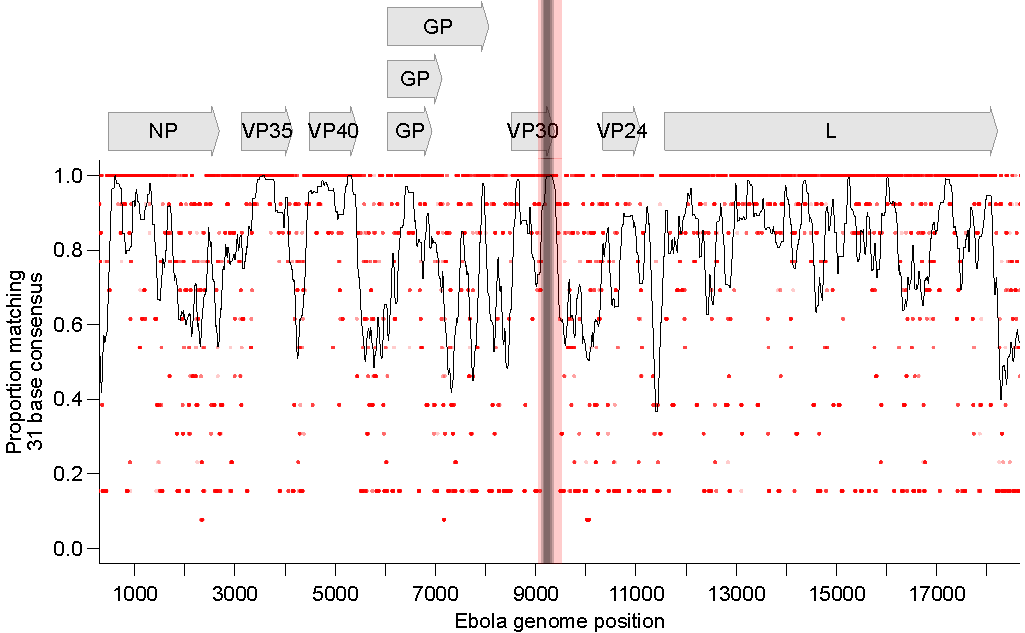
\includegraphics[width=.6\textwidth]{ebolaConsensus.pdf} %REMOVE%
		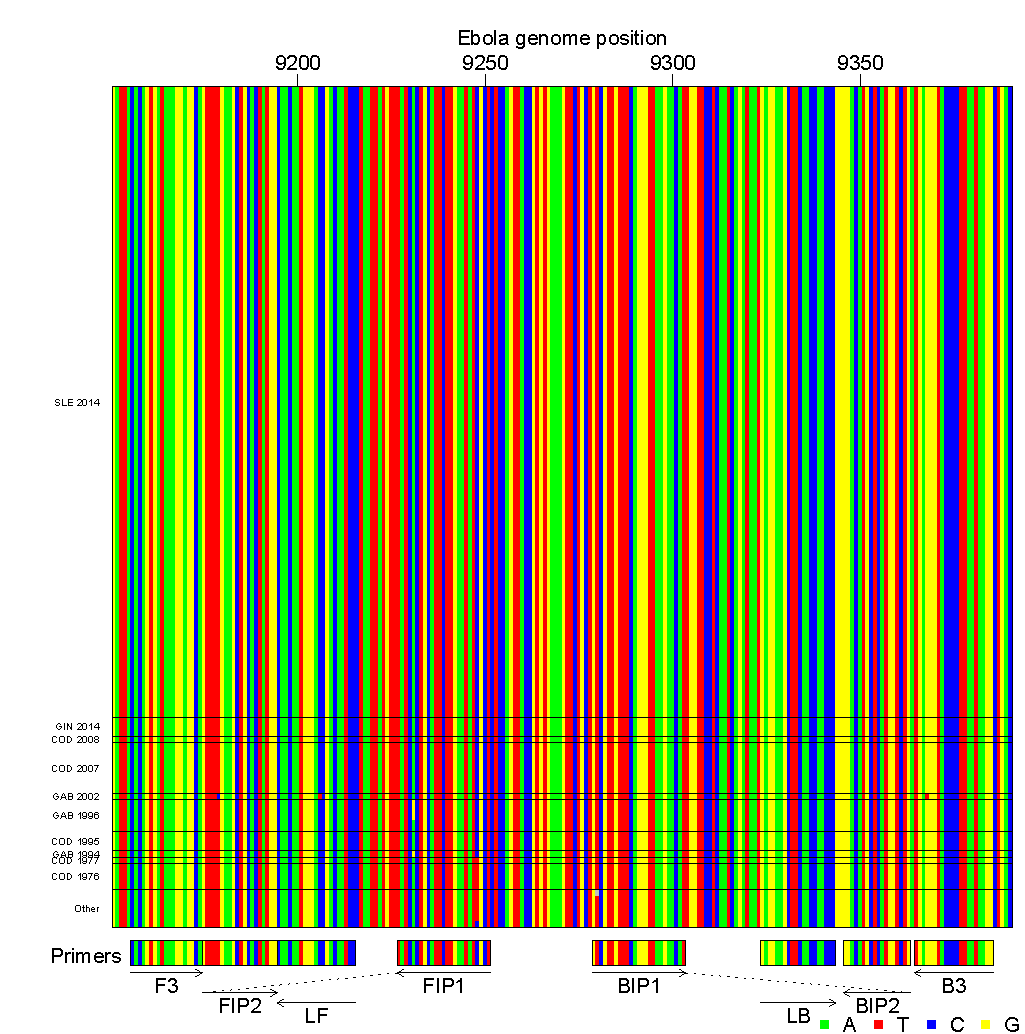
\includegraphics[width=.6\textwidth]{loop_bases.pdf} %REMOVE%
		\caption[Ebola RT-LAMP primers design]{Bioinformatic analysis to design Ebolavirus RT-LAMP primers. A) Conservation of sequence in Ebolavirus. Ebolavirus genomes (n = 131) from Genbank and sequences from the recent Zaire Ebolavirus outbreak \citep{Gire2014} were aligned and conservation calculated. The x-axis shows the coordinate on the Ebola genome, the y-axis shows the proportion of sequences matching the consensus for each 21 base segment of the genome (red points). The black line shows a 101 base sliding average over these proportions. The vertical red shading shows the region targeted for LAMP primer design that was used as input into the EIKEN primer design tool and grey shading indicates the area covered by the optimized primer set. Numbering is relative to the Ebola Mayinga sequence. B) Aligned genomes, showing the locations of the LAMP primers. Sequences in the grey-shaded region in A are shown, with DNA bases color-coded as shown at the lower right. Each row indicates an Ebolavirus sequence and each column a base in that sequence. Horizontal lines separate Ebolavirus outbreaks (SLE: Seirra Leone, GIN: Guinea, COD: DR Congo, GAB: Gabon). Arrows indicate the strand targeted by each primer. Primers targeting the negative strand of the virus are shown as reverse compliments for ease of viewing.}
		\label{figEbolaConsensus}
	\end{figure}

\subsection{Conclusions}
	These studies contribute to the study and treatment of HIV-1 by revealing aspects of latency, expression and host response. They highlight the importance of primary cell models and the effects that host cell can have on viral processes. With rapidly increasing sequencing throughput, studies like those presented here offer the opportunity for a deeper and broader understanding of HIV-1 biology and host response and further development of diagnostics and therapeutics.

\end{document}
